% !TEX root = ../thesis.tex
\label{cha:methods}
So far, we have defined some neural network building blocks. In this chapter, we are going to introduce some methods to define models with reduced computational cost and some methods to reduce the computational cost of a defined model. After introducing each method, we are going to explain how we used them in our experiments.

\section{Pruning}
\label{sec:pruning}
Pruning aims to reduce model complexity by \textit{deleting} the parameters that has low or no impact on the result. \cite{lecun1989optimal} has shown that using the second order derivative of a parameter, we can estimate the effect it will have on the training loss. By removing parameters that have low effect on the outcome, they have reduced the computational cost of their model and increased accuracy. \cite{Hu:2016aa} has shown that there may be some neurons that are not being activated by the activation function (i.e. $\RELU$ in their case). Therefore, they count the neuron activations and remove the ones that are not being activated. Following pruning, they retrain their network and achieve better accuracy than non-pruned network. \cite{han2015learning} shows that we can prune the weights that are very close to 0. By doing that they reduce the number of parameters in some networks about 10 times with no loss in accuracy. To do that, they train the network, prune the unnecessary weights, and train the remaining network again.  \cite{tu2016reducing} shows that using Fisher Information Metric we can determine the importance of a weight. Using this information they prune the unimportant weights. They also use Fisher Information Metric to determine the number of bits to represent individual weights. Also, \cite{reed1993pruning} compiled many pruning algorithms. 

In this study, we are going to look at two types of pruning methods, pruning connections and pruning nodes.

\subsection{Pruning Connections}
This type of pruning methods reduce the number of floating point operations by removing some connections. In other words, as seen in Figure~\ref{fig:weight_pruning}, they remove individual values from weight matrices. In theory, removing such connections from a weight matrix (i.e. $\wk{k}$) could benefit the computational complexity. However, in practice, we represent the connections between layers using dense weight matrices. To be able to \textit{remove} weights in such a setting, we need to convert these dense weight matrices to sparse weight matrices. However, to our knowledge, operating with dense matrices is much faster than operating with sparse matrices, unless the sparse matrix is smaller than 90\% of the weight matrix. Because of this limitation, we will not apply this method it to directly reduce the computational cost. However, we will make use of this method when we are investigating approximation methods in Section~\ref{sec:approximation}.

To determine the nodes to be pruned, we will look at one simple criteria.

\subsubsection{Irrelevant Connections}
One way to prune weights is to remove relatively irrelevant connections. To do so, we will set a threshold and remove the absolute values below that threshold. To determine this threshold we will make use of the mean and the variance of weight matrices. By finding a different threshold for different weight matrices, we will try to maximize the efficiency of this method.

\begin{figure}[!h]
  \begin{center}
  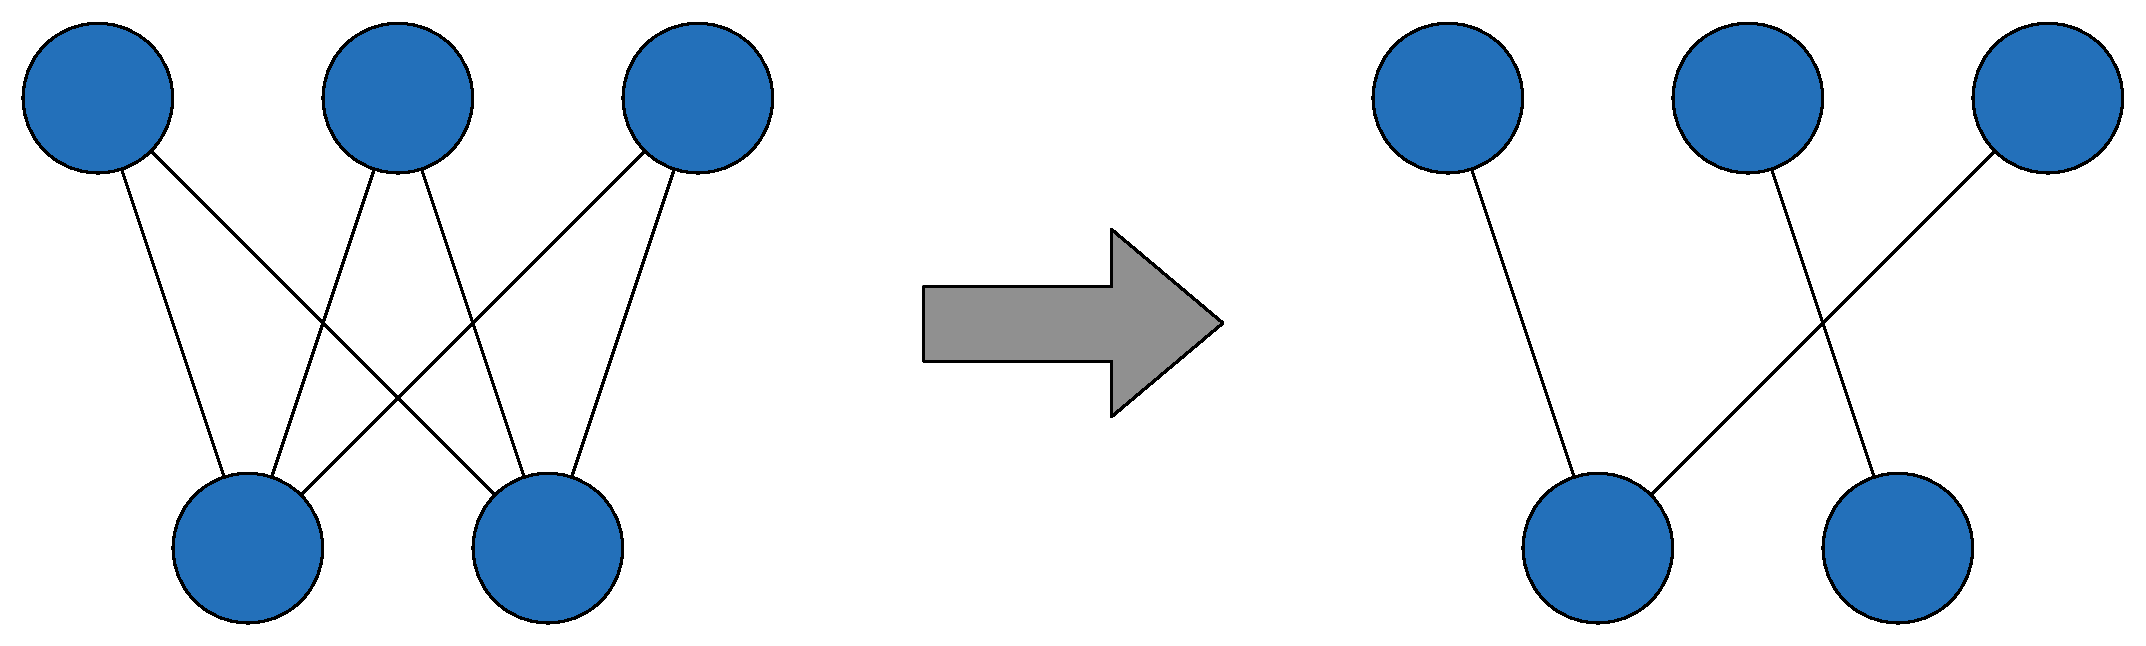
\includegraphics[width=0.5\textwidth]{images/weight_pruning.pdf}
  \end{center}
  \caption{Pruning connections of two fully connected layers. The figure on the left shows the connections before pruning, and the figure on the right shows the connections after pruning.}
  \label{fig:weight_pruning}
\end{figure}

\newpage
\subsection{Pruning Nodes}
\label{sec:pruning_nodes}
This type of pruning methods reduce the number of floating point operations by removing nodes from layers and all the weights connected to them, as seen in Figure~\ref{fig:node_pruning}. Let us assume two fully connected layers, $k$ and $k+1$. The computational complexity of computing the outputs of these two layers would be $\bigo{\FCk{k+1}(\FCk{k}(\ok{k-1})} = \bigo{\mk{k}(\mk{k-1} + \mk{k+1}}$. Assuming that we have removed a single node from layer $k$, the complexity would drop by $\mk{k-1} + \mk{k+1}$. 

\begin{figure}[!h]
  \begin{center}
  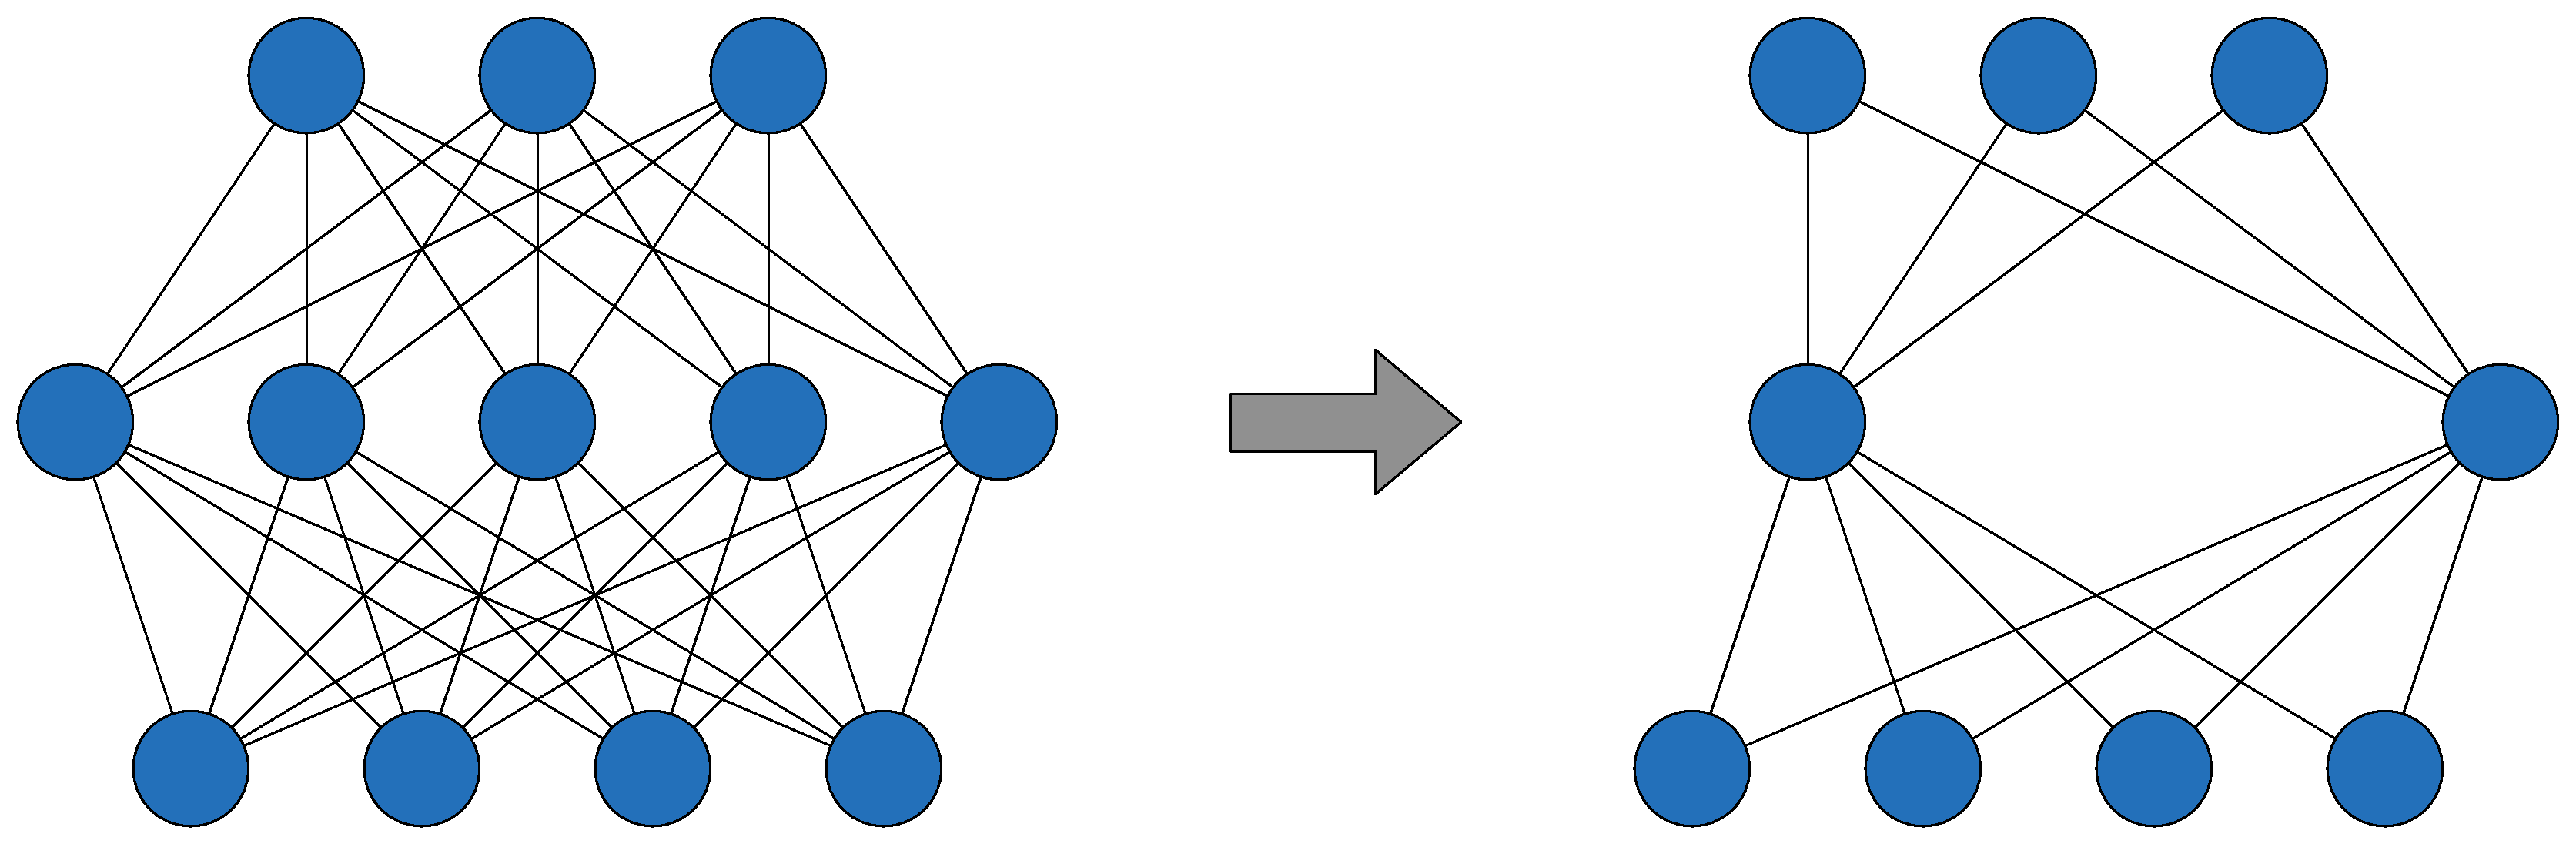
\includegraphics[width=0.7\textwidth]{images/node_pruning.pdf}
  \end{center}
  \caption{Pruning the nodes of a layer fully connected to two layers. The figure on the left shows the node structure before pruning, and the figure on the right shows the node structure after pruning.}
  \label{fig:node_pruning}
\end{figure}

Similar to the fully connected layer, a convolutional layer $k$ also contains $\mk{k}$ nodes. The only difference is, in a convolutional layer, these nodes are repeated in dimensions $H_k$ and $W_k$. Therefore, it is possible to apply this technique to convolutional layers. 

To determine the nodes to be pruned, we will look at two simple pruning criteria, activation counts and activation variance. Then we will explain the training cycles that applies pruning.

\subsubsection{Activation Counts}
We can count the activations per node to determine which nodes are not used. We can set a range using the mean and variance of activation counts and prune the nodes outside this range. By doing so, we can determine the nodes that are not frequently used or the nodes that are too frequently used.

\subsubsection{Activation Variance}
We can also collect statistics about output values per node. Using this information it is possible to determine which nodes are more important for the results by calculating the variance per node and removing the low variance nodes. 

\subsubsection{Training Cycles}
Based on these criteria, as used by \cite{Hu:2016aa} and many others, we employ training cycles. First we initialize our models with random weights. After our model converges, we collect statistics based on the selected pruning criteria. Using these statistics, we prune the model. If we have successfully pruned any nodes, we go back to the training step and keep iterating over these steps until we cannot find any nodes to prune at the end of a training cycle. The training cycles are illustrated in Figure~\ref{fig:training_cycles}.

\begin{figure}[!h]
  \begin{center}
  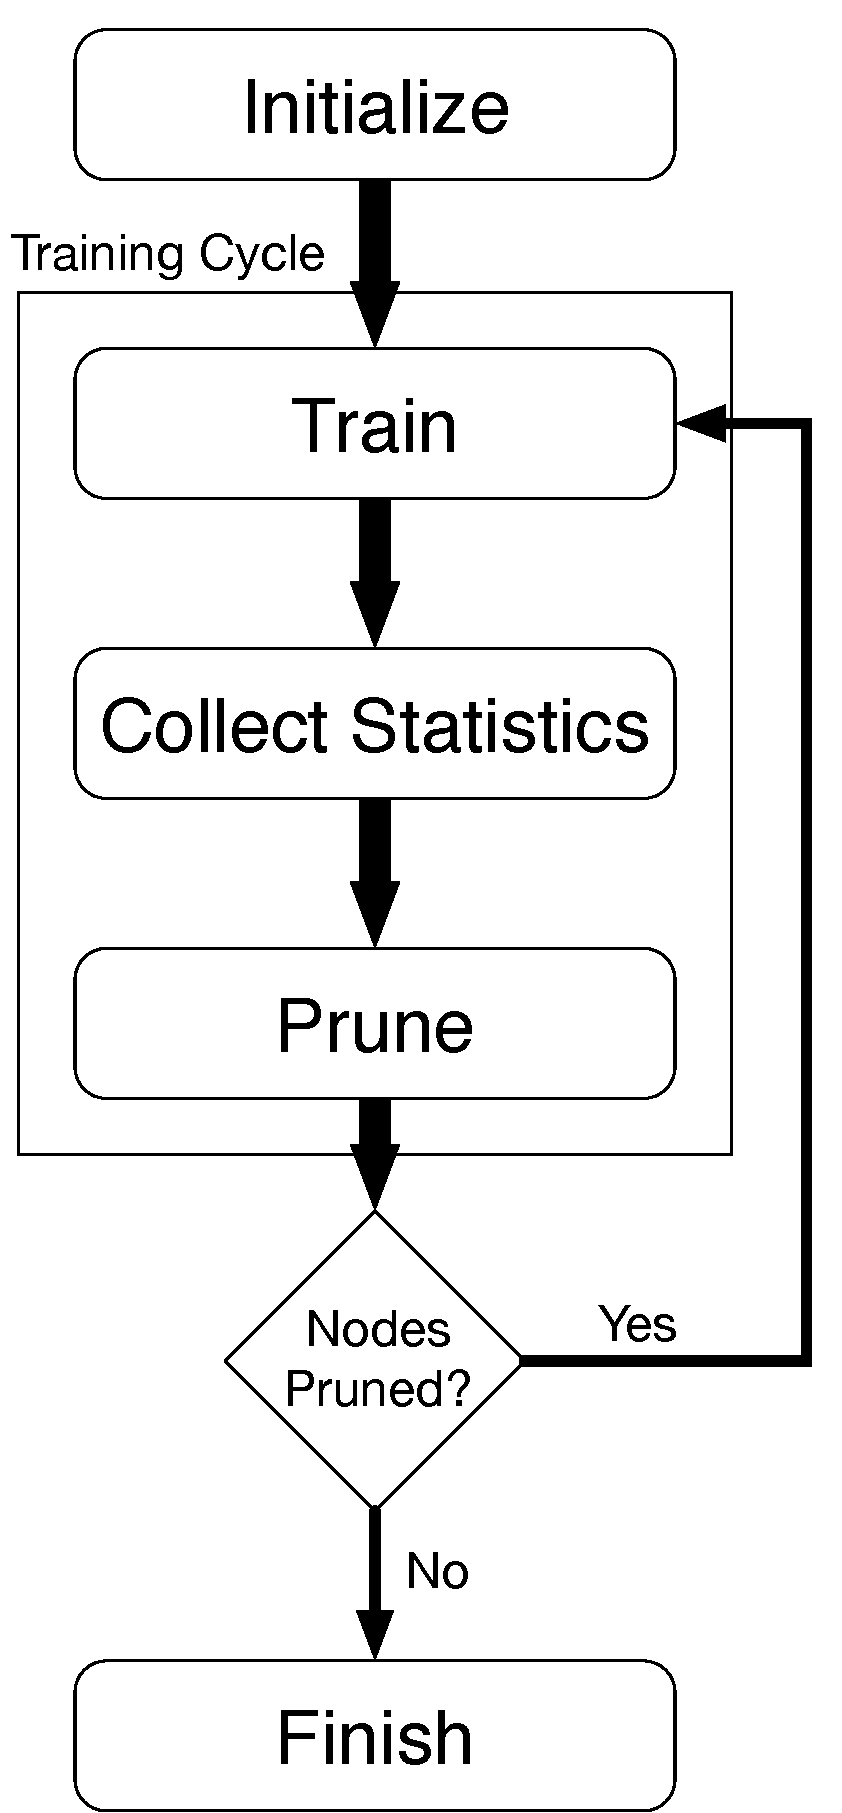
\includegraphics[width=0.5\textwidth]{images/training_cycle}
  \end{center}
  \caption{Training cycles we have defined.}
  \label{fig:training_cycles}
\end{figure}

\subsection{Experiments}
So far we have defined two pruning methods, pruning connections and pruning nodes. Since we cannot directly use pruning connections to reduce computational cost, we will focus on experimenting with pruning nodes. To be able to interpret our results, we will try to create some simple cases for which we can find the most optimum solution without using pruning. Knowing the most optimum solution for an experiment will give us a baseline to evaluate the performance of different configurations. In these experiments we are aiming to find the configurations that can achieve the best results.

\subsubsection{Fully Connected Networks}
To experiment with fully connected networks, we chose to train a neural network to \textit{predict} the summation of two inputs. As we have shown in Figure~\ref{fig:large_fc_summation}, we have defined a neural network consisting of 2 input dimensions ($\xn{n} \inreal{2}$), one fully connected layer with 1000 nodes and one fully connected output with a single node ($\yn{n} \in \realR$). We have defined the expected output as the summation of two inputs, ($\yn{n} = \xn{n,1} + \xn{n,2}$). 

Thanks to this definition, we precisely know the neural network structure that we're aiming for. As you can see in Figure~\ref{fig:optimum_fc_summation}, the neural network architecture we're aiming for has only one node in its fully connected layer. If all of the weights are equal to $1$ and all of the biases are equal to $0$ in such a setting, we can calculate the output with zero loss. To achieve such a setting, we are going to prune the nodes on that layer.

We have calculated the loss using $\RMSE$, and used Momentum Optimizer (learning rate $0.01$ and momentum $0.9$) to train the weights. We have generated $1.000.000$ samples, and trained the network with batch size $1000$.

\begin{figure}[h!]
  \begin{center}
  \begin{subfigure}{.5\textwidth}
    \begin{center}
        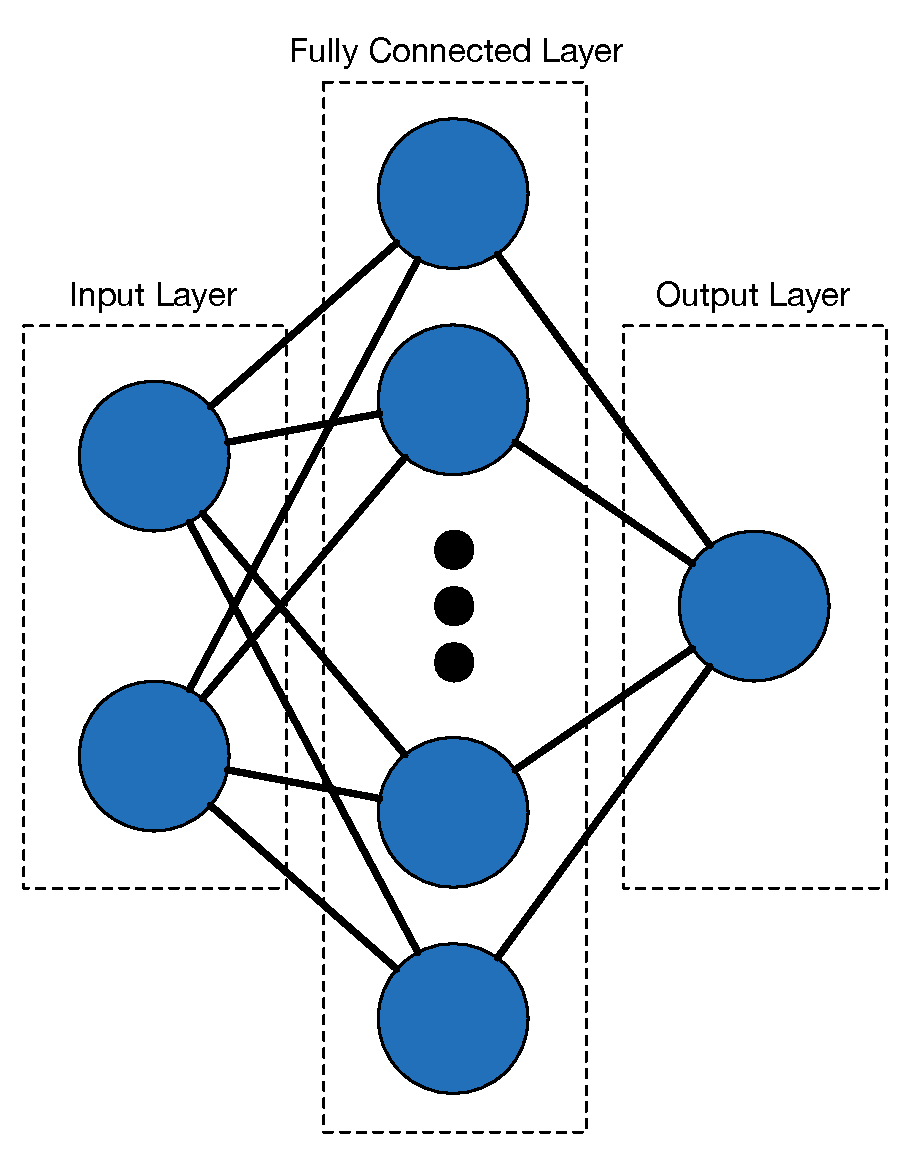
\includegraphics[width=.9\linewidth]{images/large_fc_summation.pdf}
        \caption{Initial network structure.}
        \label{fig:large_fc_summation}
      \end{center}
  \end{subfigure}% 
    \begin{subfigure}{.5\textwidth}
      \begin{center}
        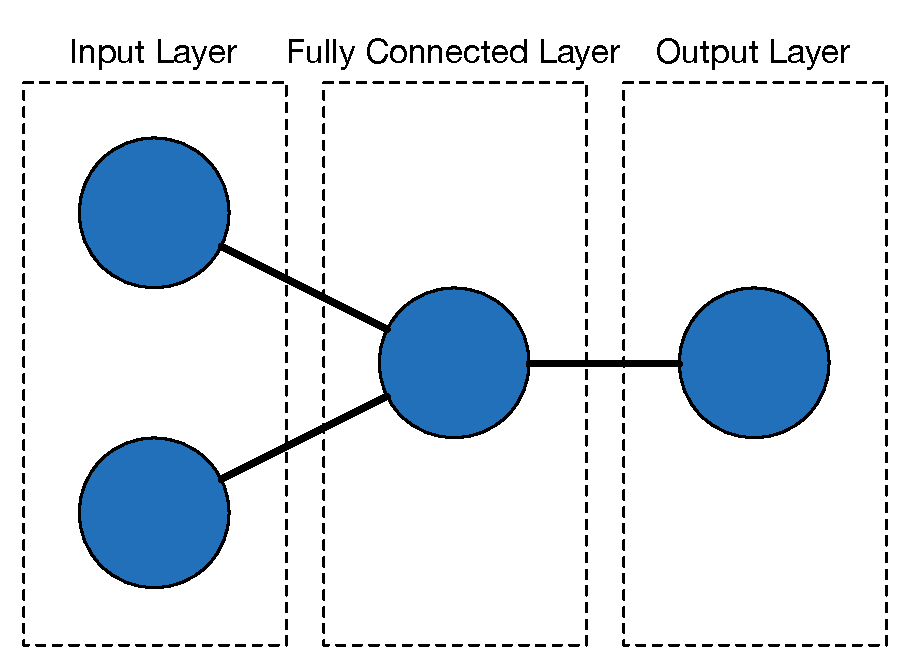
\includegraphics[width=.9\linewidth]{images/optimum_fc_summation.pdf}
        \caption{The most mathematically plausible pruned network.}
        \label{fig:optimum_fc_summation}
          \end{center}
  \end{subfigure}
  \end{center}
  \caption{(\subref{fig:large_fc_summation}) Neural network structure used to on the fully connected summation experiment, (\subref{fig:optimum_fc_summation}) the result we are trying to achieve.}
  \label{fig:fc_node_pruning}
\end{figure}

\subsubsection{Convolutional Neural Networks}
To extend our pruning experiments to convolutional neural networks, we have trained an autoencoder on MNIST dataset. 

Introduced by \cite{hinton2006reducing}, autoencoders consist of encoder and decoder blocks. Encoder blocks use convolution operations to reduce the dimensionality of input. Decoder blocks use deconvolution operation to increase the dimensionality back to it's original form. The output of encoders are approximations of the input. 

We use autoencoders because they have a clear baseline. In the baseline autoencoder, the dimensionality of the input would be equal to the output dimensions of every layer. Assuming an input $\xn{n} \inreal{ \heightk{0} \times \widthk{0} \times \mk{0}}$, the baseline autoencoder would satisfy the following equation for every layer

$$ \heightk{k}  \widthk{k} \mk{k} = \heightk{0} \widthk{0}  \mk{0} $$

Normally, an autoencoder aims to reduce the dimensionality using encoder blocks. This baseline definition is not good as an encoder, but a good comparison for our results.

We have defined our autoencoder with two encoder and two decoder layers. Each encoder layer ($\convk{1}$ and $\convk{2}$) is running a convolution with kernel size $3$ and stride of $2$. After each encoding layer, we add bias, apply batch normalization and $\RELU$ activation. Each decoding layer ($\lftk{Deconv}{3}$ and $\lftk{Deconv}{4}$) is running deconvolutions with kernel size of 3 and strides of two. After each, we add bias and apply batch normalization. The first decoding layer($\lftk{Deconv}{3}$) is followed by $\RELU$ activation and the last one is followed by $tanh$ activation. We defined the loss as the root mean square of the input and the output of the network. The initial autoencoder configuration can be seen in Figure~\ref{fig:initial_autoencoder} and the baseline autoencoder configuration can be seen in Figure~\ref{fig:baseline_autoencoder}.

\begin{figure}[!h]
    \begin{subfigure}{1\textwidth}
        \hspace{-.1\linewidth}
        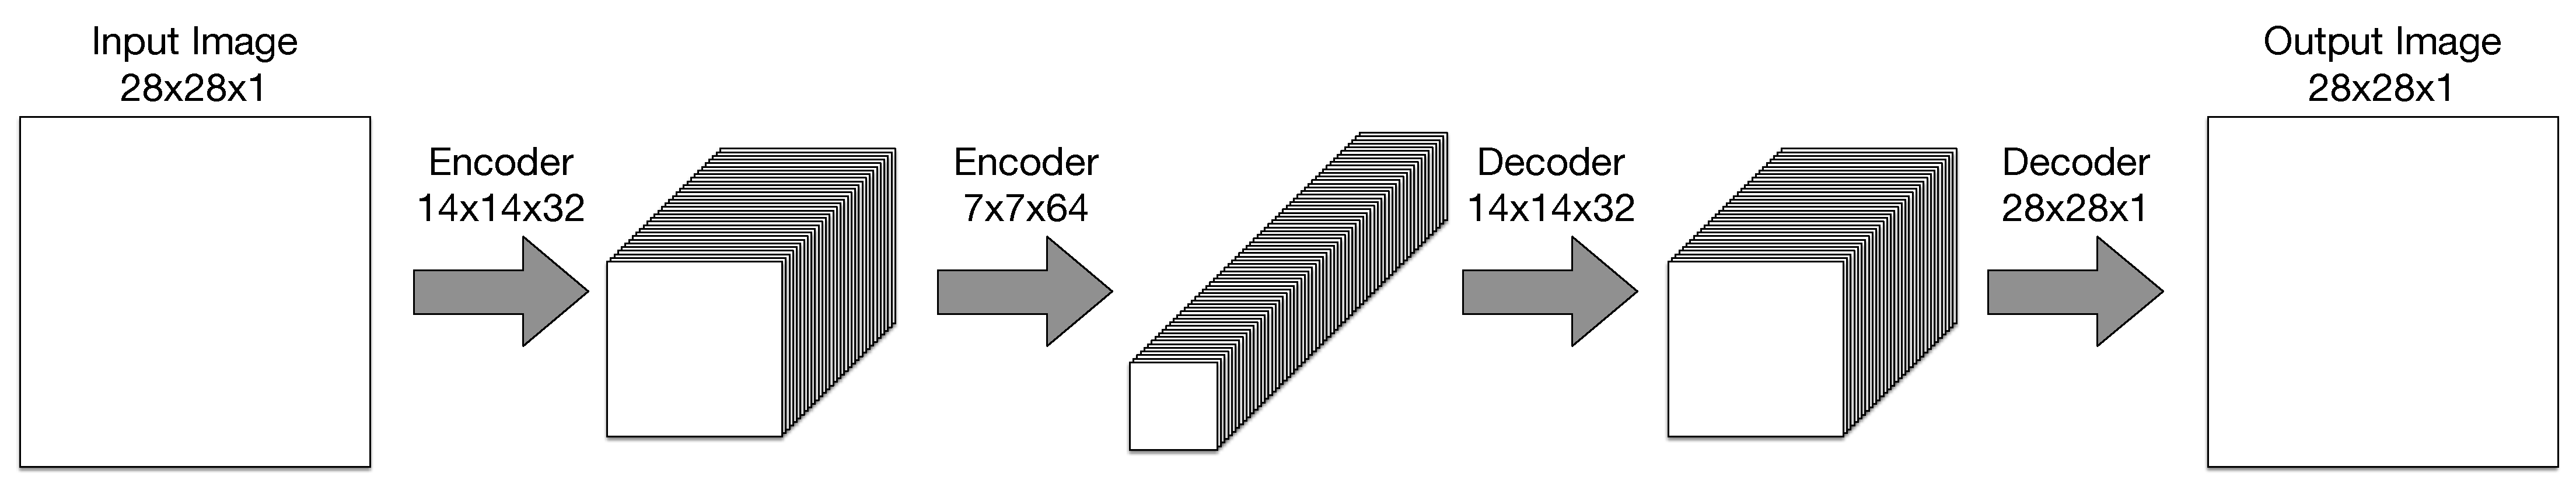
\includegraphics[width=1.2\linewidth]{images/over_parameterized_autoencoder.pdf}
        \caption{Initial autoencoder configuration.}
        \label{fig:initial_autoencoder}
    \end{subfigure}
    \begin{subfigure}{1\textwidth}
        \hspace{-.1\linewidth}
        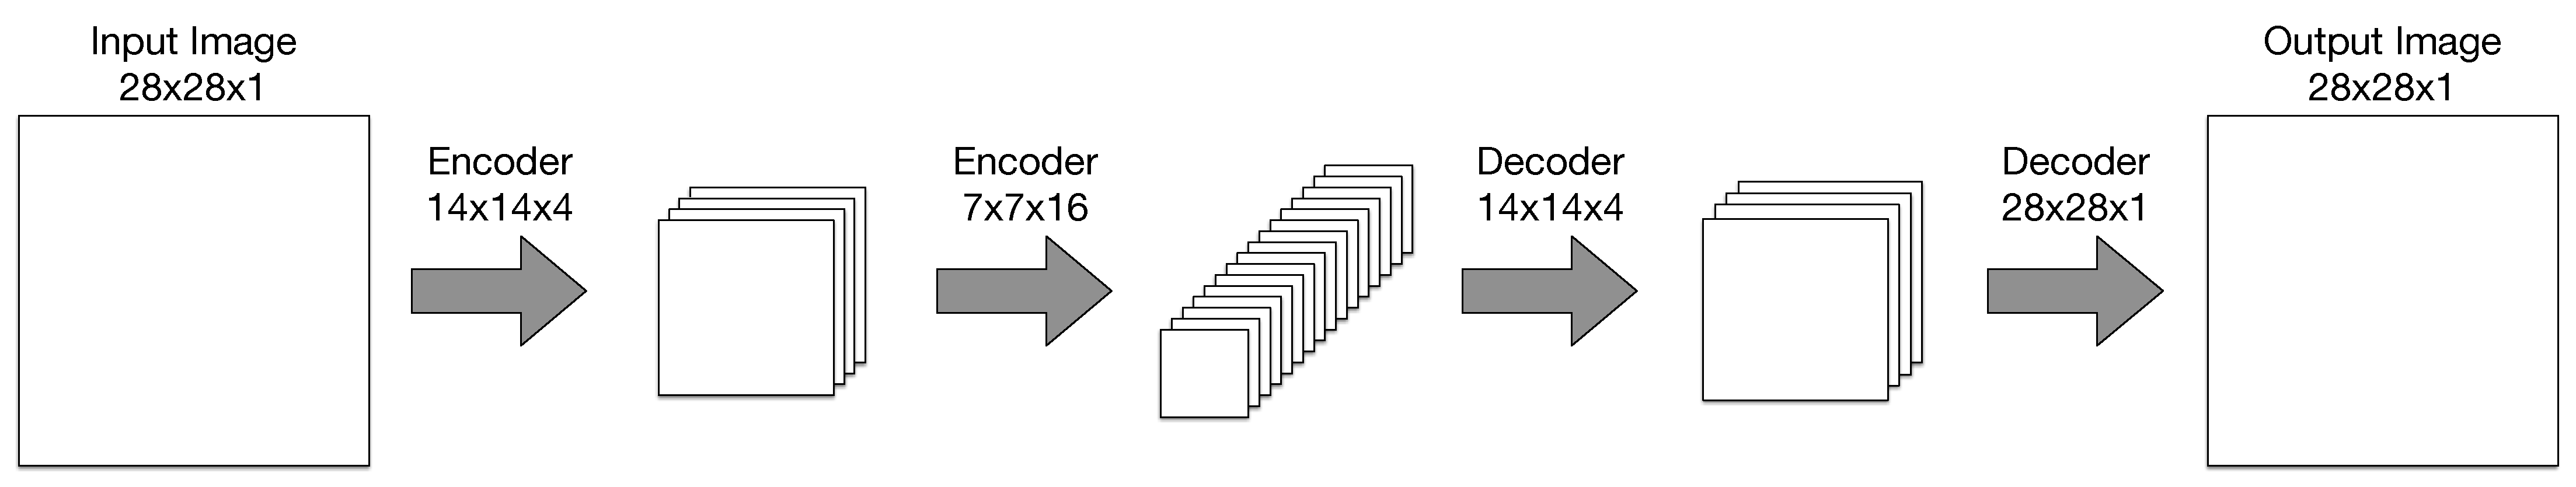
\includegraphics[width=1.2\linewidth]{images/baseline_autoencoder.pdf}
        \caption{Baseline autoencoder that doesn't reduce the dimensionality.}
        \label{fig:baseline_autoencoder}
    \end{subfigure}
    \iffalse
    \begin{subfigure}{1\textwidth}
        \hspace{-.1\linewidth}
        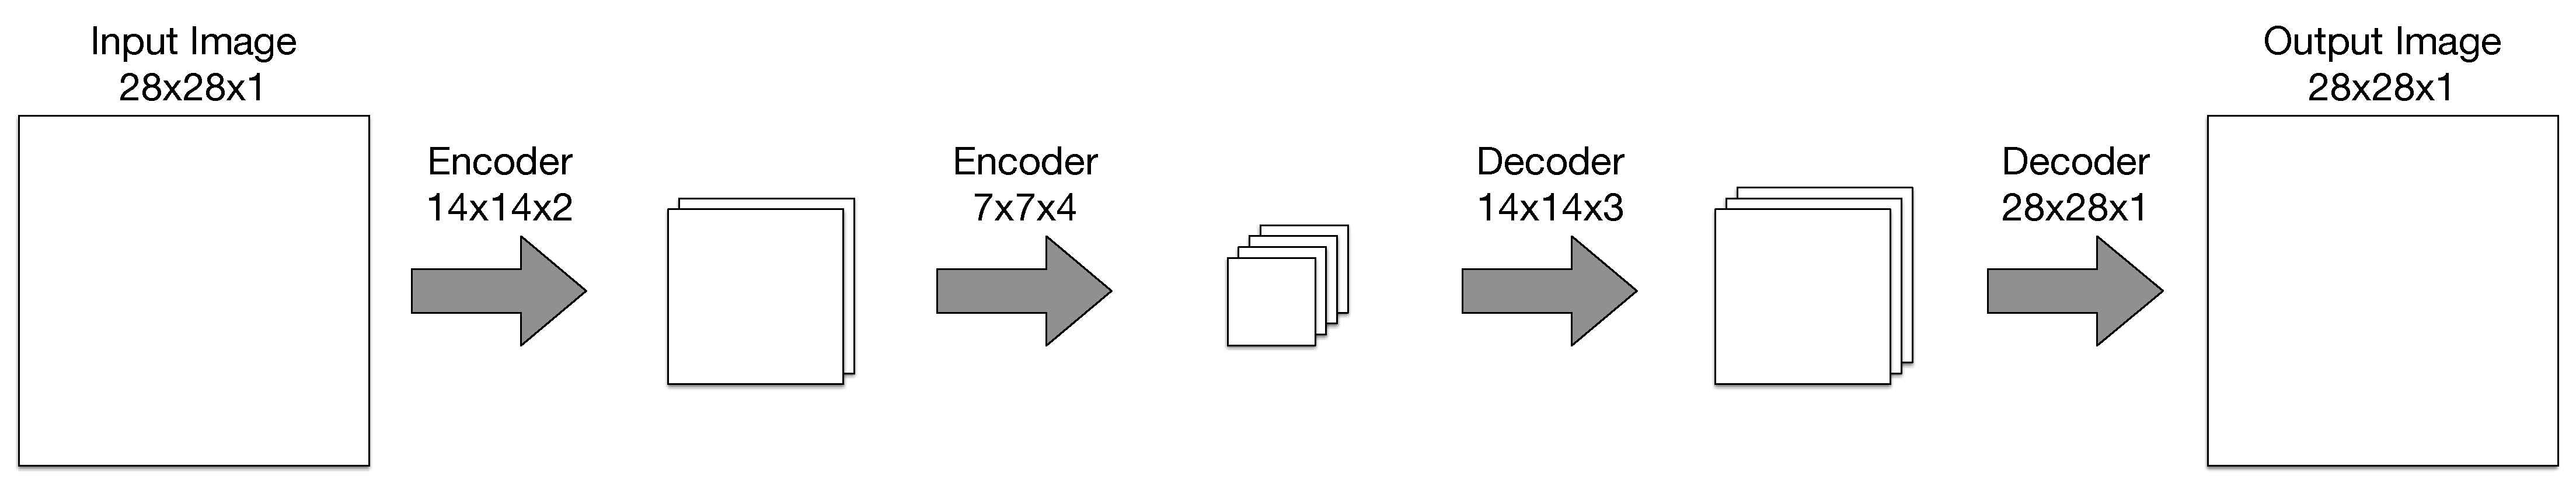
\includegraphics[width=1.2\linewidth]{images/optimum_autoencoder.pdf}
        \caption{Optimum network configuration that can perform the task.}
        \label{fig:optimum_autoencoder}
    \end{subfigure}
    \fi
    \caption{Autoencoders configurations.}
    \label{fig:autoencoders}
\end{figure}


\iffalse
\subsection{Pruning Strategies}
In this subsection we will look at the strategies we have followed to optimize the number of pruned nodes.

\subsubsection{Regularization}
In both experiments, we test no regularization, L1 regularization and L2 regularization to see how they effect pruning.

\subsubsection{Distortion}
In cases where some nodes are mostly activated together, we can assume that they are representing similar features. To prevent such cases, we tried to distort the weights between training cycles and force some difference in feature representations.
\fi

\section{Approximation Methods}
\label{sec:approximation}
In this section, we are going to look at some ways to reduce the computational cost of fully connected layers and convolutional layers by approximating their results. We will look at two types of approximation methods, factorization and quantization.

\subsection{Factorization}
Factorization approximates a weight matrix as the product of smaller matrices. As explained by \cite{zhang2016accelerating}, \cite{denton2014exploiting}, \cite{chung2016simplifying}, factorization has interesting uses with neural networks. Let us assume that we have a fully connected layer $k$. Using factorization, we can approximate $\wk{k} \inreal{\mk{k-1} \times \mk{k}}$ using two smaller matrices, $U_{\wk{k}} \inreal{\mk{k-1} \times n}$ and $V_{\wk{k}} \inreal{n \times \mk{k}}$. As shown in Figure~\ref{fig:factorization}, if we can find matrices such that $U_{\wk{k}}V_{\wk{k}} \approx \wk{k}$, we can rewrite $\FCk{k}$ as
$$\FCk{k}(o) \approx \FCkp{k}(o) = \sigma(o^T U_{\wk{k}}V_{\wk{k}} +\bk{k})$$
\begin{figure}[!h]
  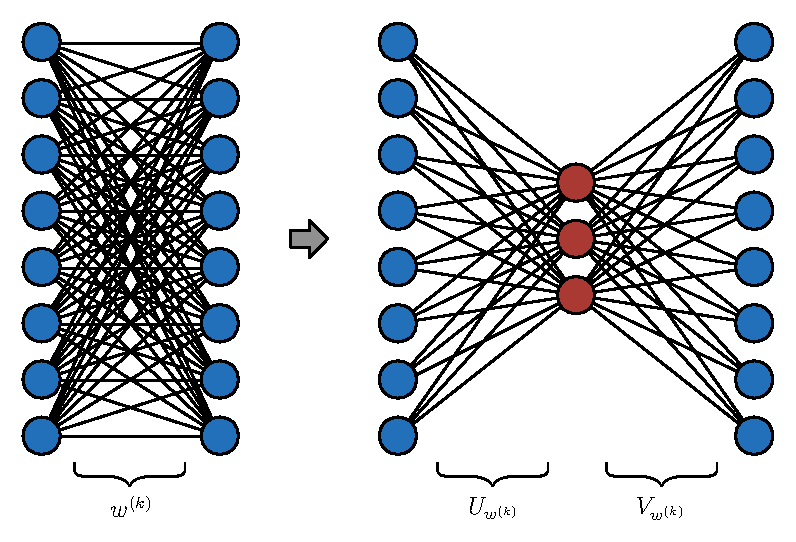
\includegraphics[width=1\textwidth]{images/factorization.pdf}
  \caption{Factorization on fully connected layers.}
  \label{fig:factorization}
\end{figure}

Therefore, we can reduce the complexity of layer $k$ by setting a sufficiently small $n$. As we have mentioned before, $\mathcal{O}(\FCk{k}) = \mathcal{O}(\mk{k-1}\mk{k})$. When we approximate this operation, the complexity becomes
$$\mathcal{O}(\FCkp{k}) = \mathcal{O}(n(\mk{k-1}+\mk{k}))$$

One thing that is similar between a convolutional layer and a fully connected layer is that both are performing matrix multiplications to calculate results. The only difference is, a convolutional layer is performing this matrix multiplication for every width and height dimension of the output layer. Therefore the same technique can be used with convolutional layers. If we apply factorization, the complexity of a convolutional layer would become
$$ \bigo{\convkp{k}} =  \bigo{\widthk{k}\heightk{k}\kernelsize^2n(\mk{k-1}+\mk{k})} $$

When factorizing fully connected and convolutional layers, if there is a good enough approximation satisfying the following equation, we can reduce the complexity without affecting the results.

\begin{equation}
\label{eq:small_n}
n < \frac{\mk{k-1}\mk{k}}{\mk{k-1}+\mk{k}}
\end{equation}

The quality of the approximation will influence how this operation affects the accuracy.

\subsubsection{SVD}
Singular Value Decomposition (SVD) (\cite{golub1970singular}), is a factorization method that we can use to calculate the elements this approximation. SVD decomposes the weight matrix $\wk{k} \inreal{\mk{k-1} \times \mk{k}}$ into $3$ parts as
$$ \wk{k} = USV^T $$
Where, $U \inreal{\mk{k-1} \times \mk{k-1}}$ and $V \inreal{\mk{k} \times \mk{k}}$ are two square matrices and $S \inreal{\mk{k-1} \times \mk{k}}$ is a rectangular diagonal matrix. The diagonal values of $S$ are called as the singular values of $\wk{k}$. Selecting the $n$ highest values from $S$ and corresponding columns from $U$ and $V$ lets us create a \textit{low rank decomposition} of $\wk{k}$ as
$$ \wk{k} \approx U'S'V'^T $$
where $U' \inreal{\mk{k-1} \times n}$, $V'^T \inreal{n \times \mk{k}}$, and $S' \inreal{n \times n}$. By choosing a sufficiently small rank ($n$) satisfying Equation \ref{eq:small_n} and setting $U_{\wk{k}}=U'S'$ and $V_{\wk{k}} = V'^T$, we can approximate the weights, and reduce the complexity of a layer. \cite{zhang2016accelerating} applies this method to reduce the execution time of a network by 4 times and increase accuracy by 0.5\%.

\iffalse
\begin{figure}[!h]
  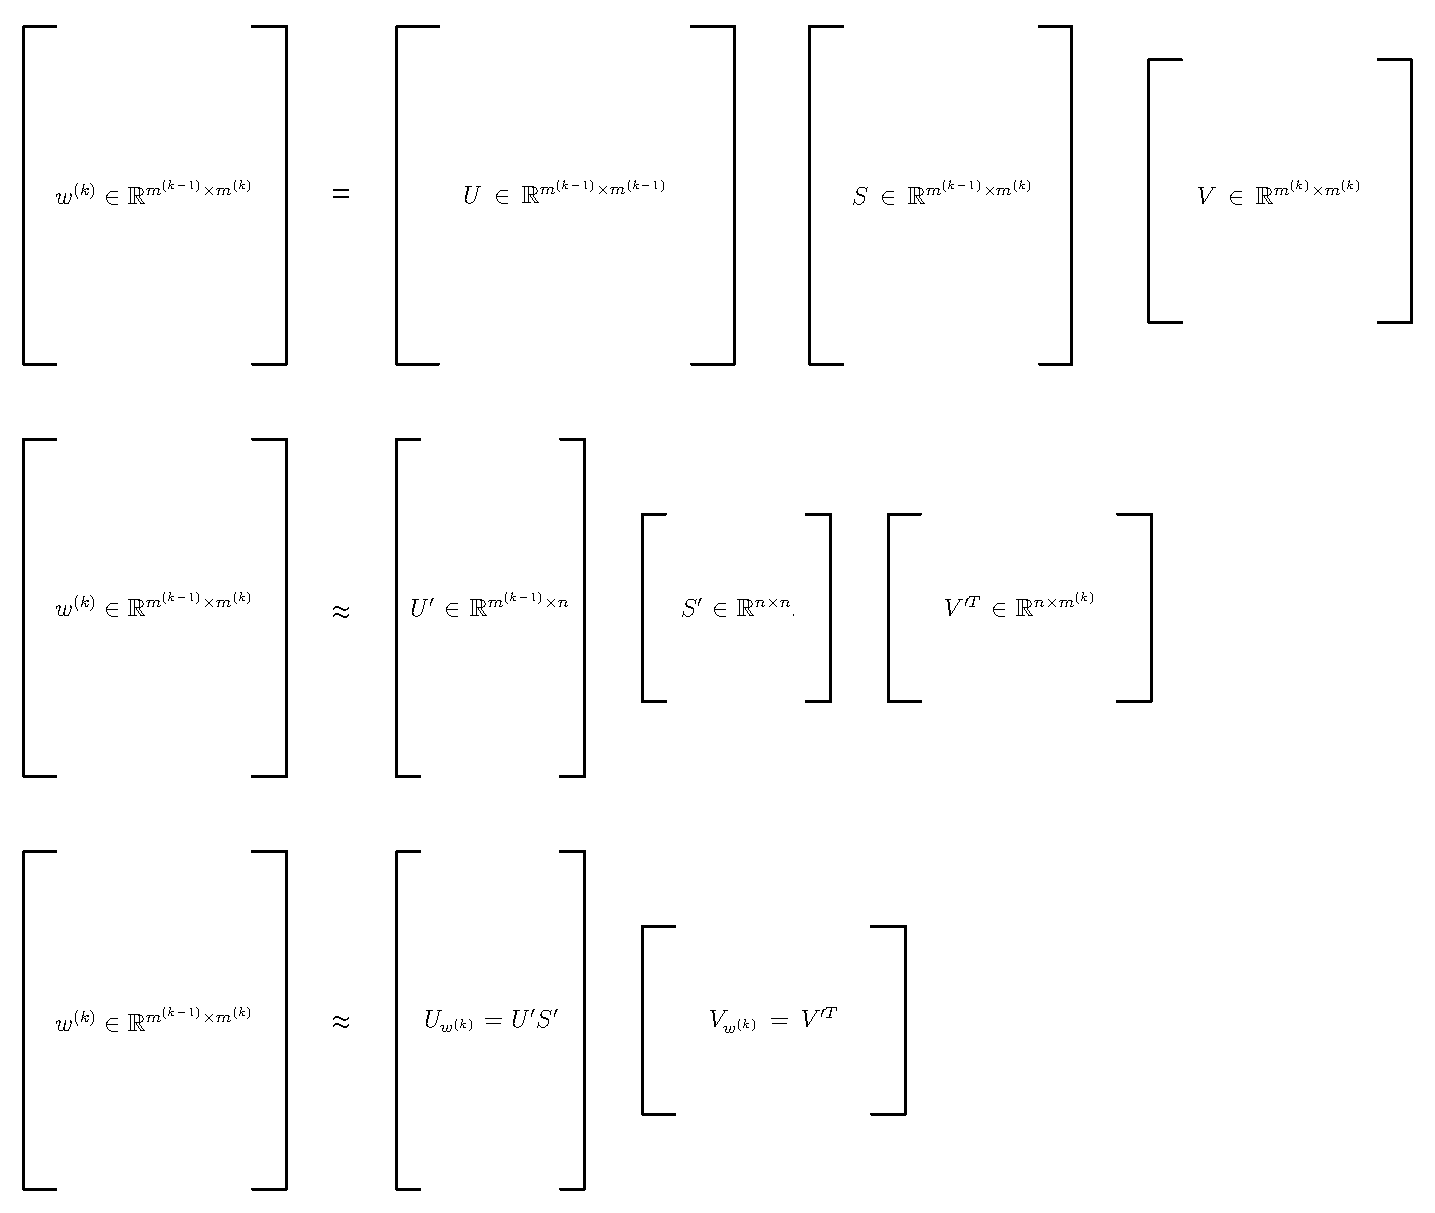
\includegraphics[width=1\textwidth]{images/svd.pdf}
  \caption{Applying SVD on a weight matrix.}
  \label{fig:factorization}
\end{figure}
\fi
\subsection{Quantization}
A floating point variable can not represent all decimal numbers perfectly. An n-bit floating point variable can only represent $2^{n}$ decimals. The decimals that can not be represented perfectly using these bits are going to be represented with some error. Quantization is the process of representing values using less bits and some error. For example, \cite{han2015deep} uses 5-bits to represent decimals, instead of 32-bit floating point variables. 

At a higher level, the computational complexity does not depend on number of bits. But if we dive deeper in the computer architecture, using less bits to represent variables provide some major advantages. As the number of bits gets smaller, the required cpu-cycles to perform an operation and the cost of transferring data from memory to cpu cache reduces. Moreover, it increases the amount of data that can fit into the cache. One disadvantage is, most architectures implement optimizations that speed up 16/32/64-bit floating point operations. By using less bits, we are giving up on these optimizations. 


\subsubsection{Weight Clustering}
Also as known as \textit{hashing trick} or \textit{feature hashing}, this method aims to represent weight matrices using a set of vaues. \cite{nowlan1992simplifying} trains their model with regular weight matrices. Once model is trained, they use clustering (i.e k-means) to find a set of weights($\all\weights' \inreal{a}$) that approximate the model. Then they store the cluster index per weight in $d^{(k)} \in \mathbb{N}^{\mk{k-1} \times \mk{k}}$. By redefining $\wk{k}_{i,j} = \all\weights'_{d^{(k)}_{i,j}}$, they perform weight clustering. 

\cite{chen2015compressing} uses a method called frequency sensitive hashing. Assuming that low-frequency weights have more importance than high-frequency weights, they cluster the weights in similar frequencies, then they create shared weights for these clusters, By doing so, they emphasize the low-frequency (high importance) features.

Please note that weight clustering methods do not necessarily reduce model complexity. However, they reduce the model size by storing indices using less bits. In theory, these methods should also provide a lower rank in low rank decomposition. 

\section{Convolution Operation Alternatives}
\label{sec:conv_alternatives}
As we have shown in the first chapter, the computational cost of convolution operation is described as the multiplication of width, height, kernel size squared, input channels and output channels. This computational cost can be quite high when we are working with large images, or large kernels, or large input and output channels. Here we will look at some alternative methods to define convolution operations with lower computational cost.
\subsection{Kernel Composing Convolutions}
As  \cite{alvarez2016decomposeme} explains, a convolution operation with a weight matrix $\wk{k} \inreal{\kernelsize \times \kernelsize \times \mk{k-1} \times \mk{k}}$, could be composed using two convolution operations with kernels $\wk{k,1} \inreal{1 \times \kernelsize \times \mk{k-1} \times n}$ and $\wk{k,2} \inreal{\kernelsize \times 1 \times n \times \mk{k}}$ as
$$ \wk{k} \approx \wk{k,1} \wk{k,2} $$
\begin{figure}[!h]
  \begin{centering}
  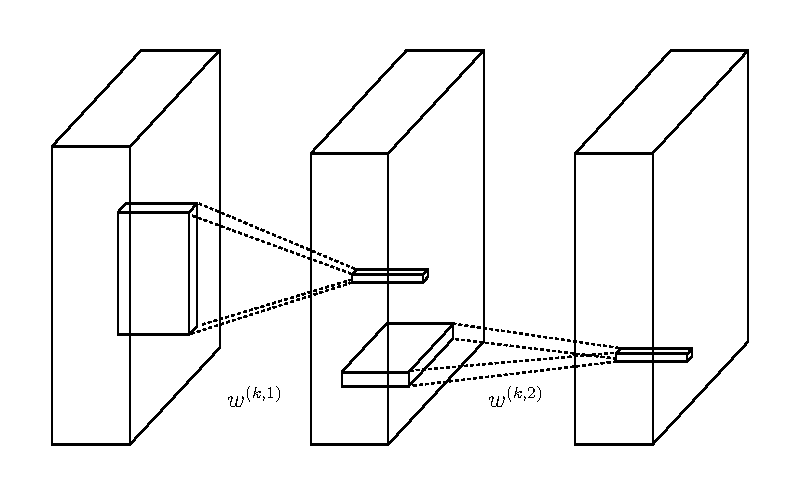
\includegraphics[width=.9\textwidth]{images/kernel_composing.pdf}
  \caption{Kernel composing convolutions visualized}
    \end{centering}
  \label{fig:depthwise_conv}
\end{figure}

Their technique, instead of factorizing learned weight matrices, aims to define weight matrices as if they were factorized and learn these values. They also aim to increase non-linearity by adding bias and activation function in between. Therefore this operation can be defined as

$$ \lfpkt{k}{KCConv}(o) = \convk{k,2}(\convk{k,1}(o))$$

As \cite{alvarez2016decomposeme} explained, their method forces the separability of the weight matrix as a hard constraint. By performing such an operation, they convert the computational complexity of a convolution operation to $\mathcal{O}(\kernelsize n(\mk{k-1} +\mk{k}))$. Suggesting that, similar to factorization methods, choosing an intermediate number of channels, $n$, satisfying
\begin{equation*}
\frac{n}{\kernelsize} < \frac{\mk{k-1}\mk{k}}{\mk{k-1}+\mk{k}}
\end{equation*}
we can represent a convolution operation with less computational complexity.


\subsection{Separable Convolutions}
Suggested by \cite{sifre2014rigid}, separable convolutions separate the standard convolution operation into two parts. These parts are called depthwise convolutions and pointwise convolutions. Separable convolutions are used by \cite{chollet2016xception}, \cite{howard2017mobilenets} and \cite{howard2017mobilenets} to reduce complexity of neural networks.
\subsubsection{Depthwise Convolution}
Depthwise convolutions (also referred to as inner convolution) apply a separate convolution operation  on every input channel. Therefore, number of output channels of a depthwise convolution is the number of input channels times the number of output channels of these inner convolutions. In other words, it results with a number of output channels that is equal to (or folds of) the number of input channels. Unless defined otherwise, we use inner convolution operations with one output channel. Therefore the number of input channels are equal to the number of output channels for our depthwise convolutions. Please see Figure~\ref{fig:depthwise_conv} for a visual explanation.

Formally, given a patch $ \pki{k-1}{(I,J)} \inreal{\kernelsize \times \kernelsize \times \mk{k-1}}$, depthwise convolution has a single weight matrix $\wk{k, dw} \inreal{\kernelsize \times \kernelsize \times \mk{k-1}}$. Let us assume that the subscripts of patch $\pki{k-1}{(I,J)}$ and weight matrix $\wk{k, dw}$ are described as $\pki{k-1}{(I,J),i} \inreal{\kernelsize \times \kernelsize \times 1}$ and $\wki{k, dw}{i} \inreal{\kernelsize \times \kernelsize \times 1}$.

\begin{figure}[!h]
\vspace{-30px}
  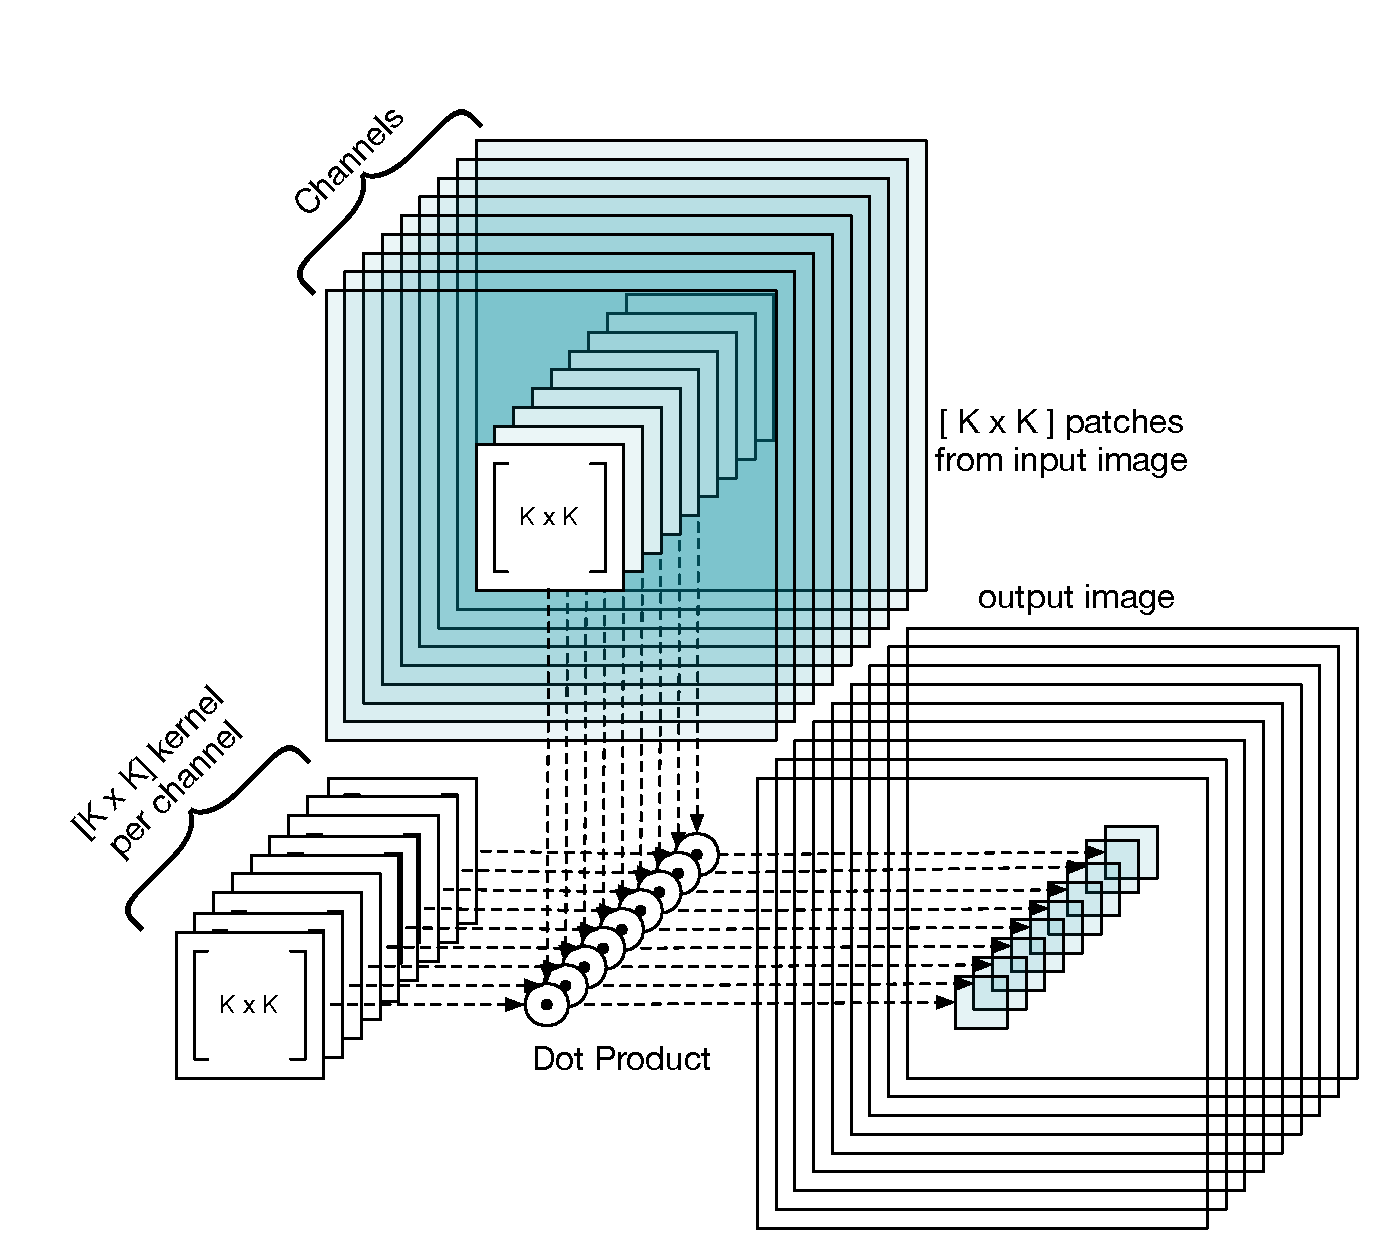
\includegraphics[width=1\textwidth]{images/depthwise.pdf}
  \caption{Depthwise convolution visualized}
  \label{fig:depthwise_conv}
\end{figure}

The depthwise convolution operation is defined as
$$ \lfkt{k}{dw} : \real{\heightk{k-1} \times \widthk{k-1} \times \mk{k-1}} \rightarrow \real{\heightk{k} \times \widthk{k} \times \mk{k-1}} $$ 
$$\lfkt{k}{dw}(\ok{k-1}) = \ok{k, dw} $$
where the output $\ok{k, dw}$ is given as
$$ \ok{k, dw} = \{ \oki{k, dw}{I,J,i} \ | \ \forall (I,J,i) (\exists \pki{k}{(I,J),i}) [\oki{k, dw}{I,J,i} = (\wki{k, dw}{i})^T \pki{k-1}{(I,J),i}  ] \} $$  % \p'_i\w'^{(k, dw)}_i \ 
In other words, depthwise convolution applies a $1 \times \kernelsize \times \kernelsize$ kernel to every $\kernelsize \times \kernelsize \times 1$ output channel to calculate every output channel of $\oki{k,dw}{I,J}$. The complexity of this operation is
$$ \mathcal{O} (\psi_k^{(dw)}) = \mathcal{O} (H_kW_kK^2\mk{k-1}) $$




\subsubsection{Pointwise Convolution}
Pointwise convolution ($\lfkt{k}{pw} : \real{\heightk{k} \times \widthk{k} \times \mk{k-1}} \rightarrow \real{\heightk{k} \times \widthk{k} \times \mk{k}}$) is a regular convolution operation with kernel size 1 ($\kernelsize = 1$). The weight matrix that we will use for this operation is $\wk{k, pw} \inreal{ 1 \times 1 \times \mk{k-1} \times \mk{k}}$. The complexity of this operation is
$$ \bigo{\lfkt{k}{pw}} = \bigo{ \heightk{k}\widthk{k}\mk{k-1}\mk{k}}$$

Since we have defined depthwise and pointwise convolutions, we can combine them to describe separable convolution function as
$$\lftk{SConv}{k} : \real{\heightk{k-1} \times \widthk{k-1} \times \mk{k-1}} \rightarrow \real{\heightk{k} \times \widthk{k} \times \mk{k}}$$
$$ \lftk{SConv}{k}(\ok{k-1}) = \lftk{pw}{k} ( \lftk{dw}{k}(\ok{k-1}) ) $$
The complexity of this operation is
\begin{equation*}
\begin{split}
\bigo{\lftk{SConv}{k}} =& \bigo{\lftk{pw}{k} + \mathcal{O} (\lftk{dw}{k}} \\
=& \bigo{\heightk{k}\widthk{k}\mk{k-1}\mk{k} + \heightk{k}\widthk{k}\kernelsize^2\mk{k-1}} \\
=& \bigo{\heightk{k}\widthk{k}\mk{k-1}(\mk{k} + \kernelsize^2)}
\end{split}
 \end{equation*}

\subsection{Non-Linear Separable Convolutions}
\cite{howard2017mobilenets} proposed that, adding batch normalization and $\RELU$ activations between depthwise and pointwise convolutions in separable convolutions would increase the model accuracy. 

\subsection{Experiments}
In general, convolution operations are expensive. Here we experiment with alternative convolution operations to see which one is the better alternative. To see the differences between these operations, we try to compare them on two tasks, one classifying MNIST dataset, the other classifying CIFAR-10 dataset. For these experiments we have defined a baseline model consisting of three convolutional layers followed by a fully connected layer. Each convolutional layer has kernel size 5. Convolutional layers are followed with bias, batch normalization, and $\RELU$ activations. First two convolution layers are followed by a max pooling layer with kernel size $2$ and strides of $2$. The third convolutional layer is followed by a global average pooling layer. We have trained the model with $\SCE$ loss and momentum optimizer with momentum $0.9$ and learning rate $0.1$ divided by 10 in steps $[20000, 30000, 40000]$. We train this model for $50000$ steps with batch size $128$. 

Overall, the layers and their outputs can be seen in Figure~\ref{fig:baseline_model}. By replacing second and third convolution operations with separable convolution, separable convolution with nonlinearity and kernel composing convolution, we obtain 3 alternative models for comparison.

We don't change the first convolution operation because using an alternative operation does not reduce the computational cost in case of $3$ input channels.

We also use a few operations using large kernels ($5\times 5$). First, kernel decomposition only provides speed up for large kernels. Second, we experiment with a small model that we can train fast, so that we can run these experiments multiple times.
\begin{figure}[!h]
  \begin{centering}
    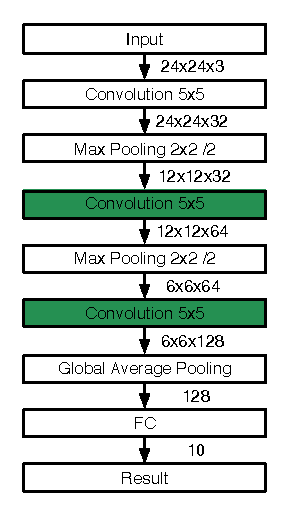
\includegraphics[width=.3\textwidth]{images/baseline_model.pdf}
    \caption{Baseline model visualised. Second and third (green) convolution operations are replaced with 3 other alternatives for comparison.}
    \label{fig:baseline_model}
  \end{centering}
\end{figure}

\section{Small Models}
Another approach to creating neural networks with low computational cost is to design smaller models. These type of models would be designed to have small input dimensions or do aggressive dimensionality reduction in first layers, use alternative convolution operations, have fewer layers and/or have less number of features per layer. For example, \cite{howard2017mobilenets} introduced a series of models with varying input dimensions and number of features. Here, we will define and train some small models for CIFAR-10 and ImageNet datasets. While defining our model, we will make use of the knowledge we have gained from the experiments we ran in Section~\ref{sec:conv_alternatives}. We will also use the methods we introduced in Sections~\ref{sec:approximation} and~\ref{sec:pruning} and try to make our models even smaller.

\subsection{Models}
Both models that we have defined were inspired by the \cite{He:2015aa} which introduces a connection that improves the performance of a neural network. Before going into the details of our models, we will explain the concepts introduced by \cite{He:2015aa}.

\subsubsection{Residual Networks}
\cite{He:2015aa} introduced residual connections and they called the convolutional neural networks having these connections as residual networks (ResNet). They show that residual connections improve the network performance. According to their results, as the network gets deeper, the effect of adding residual connections increases. \cite{He:2015aa} trains neural networks up to 1000 layers.

However, using residual connections, \cite{Zagoruyko:2016aa} achieves a better performance by increasing the number of features per layer, instead of adding more layers to ResNets. In other words, they show that having wider and shallower networks works better than having narrower and deeper networks. They use a ResNet with 16 wide layers to outperform the original 1000 layer ResNet model in various tasks. 

Since residual connections increase the performance of a given network with very little overhead, we will make use of them and see how they perform in small models.

\subsubsection{Definition of Residual Connections}
Let us assume \textit{blocks} to be repeated groups of consecutive layers in a neural network and define them as we have defined layers, so that the output of a block is $\ok{b}$ and the function(layers) that this block applies is $\lfk{b}$. We create a residually connected block when we add the input of a block to the output of the last layer in the block to calculate the input of the next block. Let us assume a block $b$ with input $\ok{b-1} \inreal{\mk{b-1}}$ and output  $\ok{b} \inreal{\mk{b}}$. We call this block residually connected when ${\ok{b}} = \ok{b-1} + \lfk{b}(\ok{b-1})$. 

\iffalse
\subsubsection{Vanishing Gradient}
Residual connections allow us to train deeper networks by preventing the vanishing gradient problem. As we increase the number of layers in a neural network, the gradient values for weights in the former layers start getting smaller and smaller. They get so small that they become irrelevant and do not change anything. Residual connections increase the effect of deeper layers on the output. Therefore, their gradients do not vanish because they have significant contribution to the result.

In case of a set of residually connected blocks from block $a$ to block $b$. The output of layer $b$ would be equal to
$$ \ok{b} = \lfk{b}(\ok{b-1}) + \sum_{k=a}^{b-1} \ok{k} $$
Since the output of a residually connected block includes the independent outputs of former residually connected blocks, the derivative of such a block will include the independent derivatives of former blocks. Therefore, the gradient of the output of a residually connected block will contain the gradients of to all former residually connected blocks. As \cite{veit2016residual} showed, these direct terms in the gradient are resolving the vanishing gradient problem.
\fi
\subsubsection{Residually Connected Block Types}
\cite{He:2015aa} introduced two types of residually connected blocks. The first is called a \textit{residual block}, consisting of two convolution operations and a residual connection between the input and the output of the block. The second is called a \textit{residual bottleneck block}, consisting of three convolution operations. First reducing number of channels with a one by one kernel, second applying a three by three kernel, third applying another one by one kernel to increase the number of dimensions. They have used residual blocks to train networks up to 34 layers. For networks having 50 or more layers, they have used the residual bottleneck block. Their 50 layer network using residual bottleneck blocks achieves $22.85\%$ top-1 error rate on ImageNet dataset, their 34-layer network using residual blocks achieves $25.3\%$ top-1 error rate.
\begin{figure}[h!]
  \begin{center}
  \begin{subfigure}{.5\textwidth}
    \begin{center}
        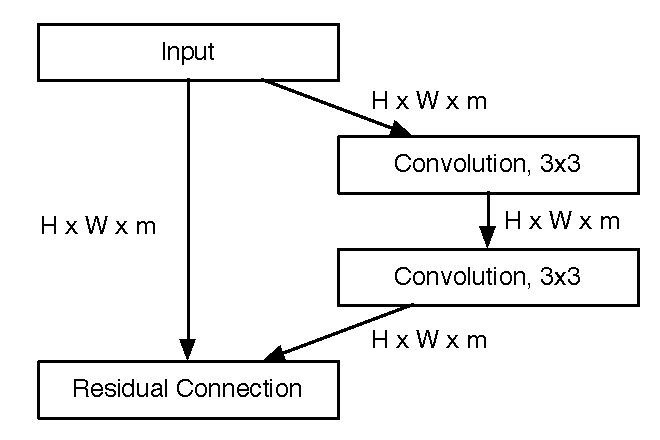
\includegraphics[width=.9\linewidth]{images/residual_block.pdf}
        \caption{A residual block.}
        \label{fig:residual_block}
      \end{center}
  \end{subfigure}% 
    \begin{subfigure}{.5\textwidth}
      \begin{center}
        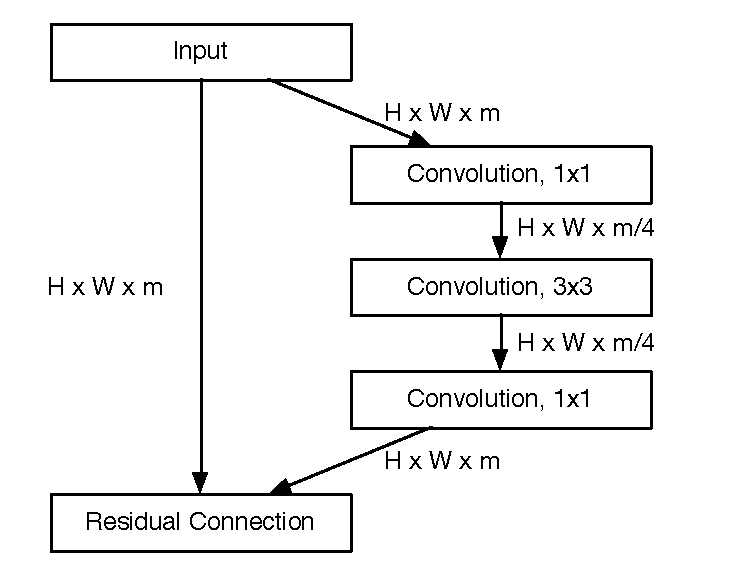
\includegraphics[width=.9\linewidth]{images/residual_bottleneck.pdf}
        \caption{A residual bottleneck block. }
        \label{fig:residual_bottleneck_block}
          \end{center}
  \end{subfigure}
  \end{center}
  \caption{Residually connected blocks, visualized as proposed by \cite{He:2015aa}. $\RELU$ non-linearity, batch normalization and identity mappings hidden for simplicity.}
  \label{fig:residual_blocks}
\end{figure}
For our models we chose to use the residual blocks. $1 \times 1$ convolutions in residual bottleneck blocks are relatively more expensive and we cannot reduce their cost using an alternative operation. Furthermore, residual bottleneck blocks are not a good fit for networks with less layers because they do not expand the receptive field as aggressively as residual blocks.

\subsubsection{Separable Residual Blocks}
To create separable residual blocks, we have replaced the convolution layers with separable convolution layers in residual blocks. Following \cite{He:2015aa}, \cite{he2016identity} proposed that using full pre-activation residual connections increases the model performance. This type of residual connections residually connect the outputs before batch normalization and $\RELU$ activation. We have illustrated these connections with separable residual blocks in Figure~\ref{fig:full-preactivation}.

When necessary, we apply strides in the first depthwise convolution and we increase the number of channels in the first pointwise convolution. As shown in Figure~\ref{fig:full-preactivation}.

\begin{figure}[!h]
  \begin{center}
    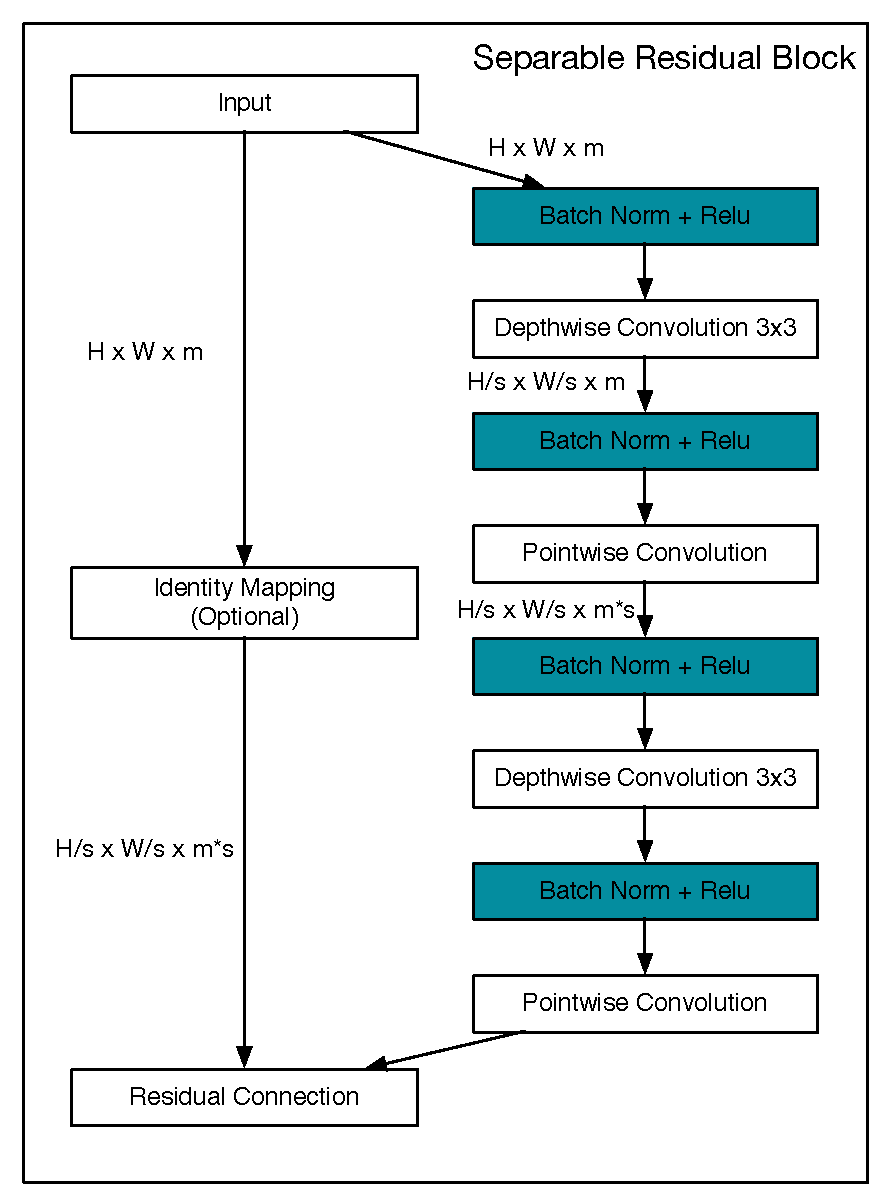
\includegraphics[width=0.6\textwidth]{images/separable_residual_block.pdf}
  \end{center}
  \caption{Full pre-activation separable residual block. $H/s$ and $W/s$ represents the strides applied to height and width dimensions respectively. $m$ represents the output channels and $m*s$ represents multiplying number of channels by the strides. Dimensions are not shown if they do not change between two layers.}
  \label{fig:full-preactivation}
\end{figure}

\subsubsection{First Convolutional Layer}
Assume that the first layer has 3 input and 32 output channels. For this layer the number of operations for the convolution operation ($\kernelsize*\kernelsize*\mk{k-1}*\mk{k} = 3*3*3*16 = 864$) is sufficiently higher than the separable convolution alternative ($\kernelsize*\kernelsize*\mk{k-1} + \mk{k-1}\mk{k} = 3*3*3 + 3*32=123$). However, for an actual image input, separable convolution comes with a disadvantage. The channels of the input image are RGB color channels, which can not be assumed independent. Therefore, since separable convolutions start with a depthwise convolution, they assume that we can apply independent convolutions on different channels, so we think that they are inefficient for such an input.

\subsubsection{CIFAR-10 Model}
For CIFAR-10, we define a very small model consisting of a convolutional layer followed by 6 separable residual blocks.  The model is illustrated in Figure~\ref{fig:separable_resnet_cifar10}. For identity mapping we have used average pooling with strides and kernel size of two. To multiply the number of channels, we have padded the feature matrices with zeros.

\begin{figure}[!h]
  \begin{center}
    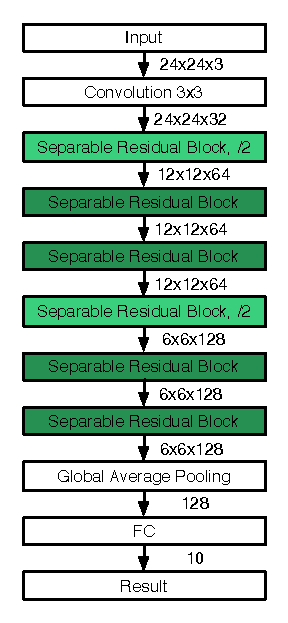
\includegraphics[width=0.38\textwidth]{images/separable_resnet_cifar10.pdf}
  \end{center}
  \caption{Model trained for CIFAR-10. Light green blocks reduce the image dimensionality by two while multiplying the number of features by 2.}
  \label{fig:separable_resnet_cifar10}
\end{figure}

We divided the dataset for 50.000 training images and 10.000 validation images. We used momentum optimizer with momentum $0.9$ and learning rates $0.1$, $0.01$, $0.001$ for steps $0$ to $40.000$, $40.000$ to $60.000$ and $60.000$ to $80.000$ respectively. We have defined the loss with $\SCE$ of the truth and prediction, with an addition of L2 norm of weights multiplied by $0.001$. We trained our model using the training images for $80.000$ steps with batch size $128$. 

We preprocess the images using the routines defined in Tensorflow tutorials\footnote{\url{https://github.com/tensorflow/models/tree/master/tutorials/image/cifar10}}\footnote{\url{https://www.tensorflow.org/tutorials/deep\_cnn\#cifar-10\_model}}. We start by taking $24 \times 24$ random crops and then we randomly flip the image to left or right. Then we randomly change the brightness and contrast. Then we normalize this image by subtracting the mean and dividing by variance by using a method called per\_image\_standardize.


\subsubsection{ImageNet Model}
We recreated the Resnet-34 using separable residual blocks instead of residual blocks. The resulting model is shown in Figure~\ref{fig:model}. For identity mappings, we have used $1 \times 1$ convolutions with strides of two because \cite{He:2015aa} shows that they work better for ImageNet dataset.

\subsubsection{Aggressive Dimensionality Reduction in ImageNet}
In \cite{He:2015aa}, models defined for ImageNet start with a $7 \times 7$ convolution with strides of two, which followed by a max pooling layer with strides of two and kernel size 2. If we think about this design choice, we see that the kernel size choice ($7 \times 7$) is to cover the receptive field to minimize the loss of information caused by two consecutive layers with strides of two. From another point of view, those two layers decrease the image size from $224 \times 224$ to $56 \times 56$. This decreases the computational cost of future layers. When we apply such a convolution, the first convolutional layer becomes very complex compared to the rest of the network. To prevent that we propose a different first layer. We change this $7 \times 7$ convolution followed by a max pooling layer with two $3 \times 3$ convolutions 
Following that, before applying the max pooling layer, we apply a $3 \times 3$ depthwise convolution that multiplies the number of channels with two. Then we apply a $1 \times 1$ convolution (pointwise) to that.  By doing so we reduce the complexity of these layers about four times. 

We trained our model in ImageNet training dataset. We used gradient descent optimizer and learning rates $0.01$, $0.001$, $0.0001$ for steps $0$ to $150.000$, $150.000$ to $200.000$ and $250.000$ to $300.000$ respectively. We have defined the loss with $\SCE$ of the truth and prediction, with an addition of L2 norm of weights multiplied by $0.001$. We train our model using the training images with batch size $128$.

We preprocess images using the routines defined for open sourced Tensorflow implementation of inception network\footnote{\url{https://github.com/tensorflow/models/blob/master/slim/preprocessing/inception_preprocessing.py}}. We start by creating a new random bounding box overlapping with the original bounding box and make sure that 0.1 of the bounding box is inside our new bounding box. Then we crop this new bounding box and resize it using bilinear resizing algorithm. Then we randomly flip it to left or right. Then we distort the colors using random brightness and saturation. Then we normalize this input to the range of $[-1,1]$ by subtracting 0.5 and multiplying by 2. 

\begin{figure}
\vspace{-65px}
  \begin{center}
        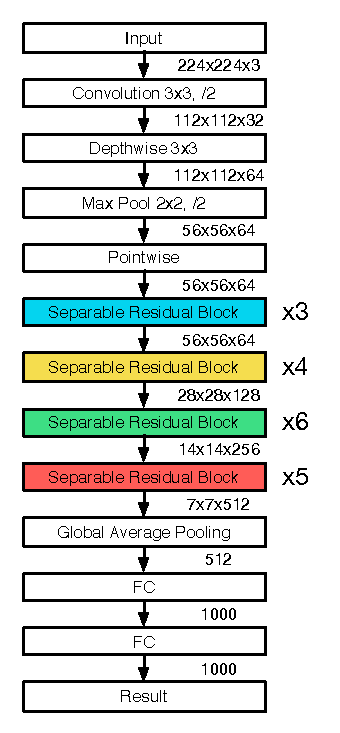
\includegraphics{images/separable_resnet.pdf}
  \end{center}
  \caption{Resnet-34 recreated using separable residual blocks and proposed input layers. $\RELU$ and Batch Normalization operations are hidden. Dimensionality is reduced in the first block of second (yellow), third(green) and fourth(red) repeated separable residual blocks.}
  \label{fig:model}
\end{figure}

After training these models, we try to apply the methods we have defined in Sections~\ref{sec:pruning}, and~\ref{sec:approximation} to see how they perform with small models.
\subsection{Pruning Small Models}
To be able to prune nodes on these models, we have defined two new pruning routines.
\subsubsection{Pruning Residual Connections}
The addition operation in the residual block creates a one-to-one relationship between the output channels of different blocks. With the existence of such a relationship, it is not possible to prune a residual block's output nodes without pruning the former or latter blocks. Therefore, we group the separable residual blocks that are residually connected with same dimensions or without identity mappings and refer to them as directly connected (in Figure \ref{fig:model}, residual blocks represented with the same colors are directly connected). Then, using a pruning criteria, we calculate the channels to keep for the input and output of every residual block. We union the nodes to be kept in those layers and prune the remaining nodes from the inputs and outputs of the directly connected residual blocks. We also prune the pointwise convolutions within residual blocks separately. 

\subsubsection{Pruning Depthwise Convolutions}
Since depthwise convolutions multiply the number of channels (nodes) by a number, their number of output channels are dependent on their number of input channels. Therefore, if the output channels of the previous layer are pruned, the corresponding input channels of the next layer should also be pruned.

\subsection{Approximating Small Models}
\label{sec:factorization}
We apply pruning connections and weight clustering before factorization to be able to reduce the computational complexity as much as possible.

\subsubsection{Pruning Connections}
We set weight values that are smaller than a threshold to 0. Despite the fact that this operation does not change computational complexity, when combined with factorization, it increases the number of zeros within the matrix. Therefore it helps with finding a lower rank.

\subsubsection{Weight Clustering}
We round the weights after the second decimal. This is a very basic method of weight clustering, however it may help finding a lower rank. 

\subsubsection{Factorization}
We factorize the trained, pruned and rounded weights using SVD. We can not apply this method to depthwise convolution operation. So we only factorize the convolution, pointwise convolution and fully connected weights. To do that, we calculate $U$, $S$ and $V$ for each of the weight matrices. We lower the rank of the decomposition by one. Then, we calculate the approximation error using mean squared error between the original matrix and the low rank weight matrices. We chose this method because it scales for the number of parameters in the weight matrix. We keep reducing the rank by 1 while the approximation error is above the predefined error threshold. When the error threshold is reached, we check if this low rank decomposition would actually reduce the complexity. If it does, we apply factorization. Otherwise we use the original weights.

\subsubsection{Quantization}
We quantize the weights from 32-bits to 8-bit and run performance and accuracy benchmarks.

\iffalse
\section{Benchmarking}
We benchmark our models on a \textit{One Plus X}\footnote{\url{https://oneplus.net/x/specs}} mobile device, equipped with a \textit{Snapdragon 801}\footnote{\url{https://www.qualcomm.com/products/snapdragon/processors/801}} chipset. Our benchmarks consist of running consecutive inferences on a model, for a period of time. While those inferences are running, we collect hardware statistics using simpleperf\footnote{\url{https://android.googlesource.com/platform/prebuilts/simpleperf/}}. Simpleperf lets us collect the hardware level performance statistics for a given process.

Our benchmarking app uses a static input image (with dimensions depending on the model). So that we can ignore the overhead of pre-processing. Also, we perform no post-processing. Doing so, we try to avoid the effects of any other computation that could change the benchmark results. 

We ran this benchmarking tool for various models. Since running the benchmark does not require a trained network, we could easily generate multiple models and benchmark them. These models include; Inception-Resnet v2 (\cite{DBLP:journals/corr/SzegedyIV16}), Inception v1 (\cite{Szegedy:2014aa}), Inception v2 (\cite{Szegedy:2014aa}), Inception v3 (\cite{Szegedy_2016_CVPR}), Inception v4 (\cite{DBLP:journals/corr/SzegedyIV16}), VGG-19 (\cite{Simonyan:2014aa}), ResNet-50, ResNet-101, ResNet-152 and ResNet-200 (\cite{He:2015aa}, \cite{he2016identity}) and Mobilenet (\cite{howard2017mobilenets}).  
\fi

\newpage
\section{Experiments}
In Table~\ref{tbl:experiments} we provide a summary of the experiments we ran.
\begin{table}[!h]
\hspace{-35px}
\begin{tabular}{|l|l|l|l|}
\thead{Method} & \thead{Model} & \thead{Dataset(s)} & \thead{Variables} \\ \hline
Pruning Nodes & fully connected & summation & \begin{tabular}[c]{@{}l@{}}regularization, \\ distortion, \\ activation counts, \\ activation variance\end{tabular} \\ \hline
Pruning Nodes & autoencoder & MNIST & \begin{tabular}[c]{@{}l@{}}regularization, \\ distortion, \\ activation counts, \\ activation variance\end{tabular} \\ \hline
Convolution Alternatives & baseline model & \begin{tabular}[c]{@{}l@{}}CIFAR-10\\ MNIST\end{tabular} & \begin{tabular}[c]{@{}l@{}}convolution, \\ kernel composing, \\ separable \\ non-linear separable \end{tabular} \\ \hline
Small Models & CIFAR-10 Model & CIFAR-10 & \begin{tabular}[c]{@{}l@{}}Number of layers, \\ number of features\end{tabular} \\ \hline
Small Models & ImageNet Model & ImageNet &  \\ \hline
\begin{tabular}[c]{@{}l@{}}Approximation Methods $+$\\ Pruning Connections\end{tabular}  & CIFAR-10 Model & CIFAR-10 & \begin{tabular}[c]{@{}l@{}}Error Threshold\\ Pruning Threshold\end{tabular}  \\ \hline
\end{tabular}
\caption{A summary of all experiments we ran.}
\label{tbl:experiments}
\end{table}
\iffalse

\begin{verbatim}
Performance counter statistics:

     2,589,237,398  L1-dcache-loads           # 940.825 M/sec       (14%)
                 0  L1-dcache-load-misses     # 0.000 /sec          (100%)
     3,393,233,002  L1-dcache-stores          # 980.415 M/sec       (17%)
                 0  L1-dcache-store-misses    # 0.000 /sec          (100%)
     2,404,509,748  L1-icache-loads           # 576.568 M/sec       (21%)
                 0  L1-icache-load-misses     # 0.000 /sec          (100%)
     2,919,824,326  L1-icache-stores          # 597.244 M/sec       (24%)
                 0  L1-icache-store-misses    # 0.000 /sec          (100%)
     5,798,305,546  dTLB-loads                # 1.023 G/sec         (28%)
     5,037,941,181  dTLB-stores               # 1.024 G/sec         (25%)
        68,593,055  iTLB-loads                # 16.289 M/sec        (21%)
        56,479,236  iTLB-stores               # 16.014 M/sec        (18%)
       337,848,194  branch-loads              # 121.453 M/sec       (14%)
                 0  branch-load-misses        # 0.000 /sec          (100%)
       408,888,494  branch-stores             # 115.616 M/sec       (18%)
                 0  branch-store-misses       # 0.000 /sec          (100%)
                 0  node-loads                # 0.000 /sec          (21%)
                 0  node-load-misses          # 0.000 /sec          (100%)
                 0  node-stores               # 0.000 /sec          (25%)
                 0  node-store-misses         # 0.000 /sec          (100%)
                 0  node-prefetches           # 0.000 /sec          (28%)
                 0  node-prefetch-misses      # 0.000 /sec          (100%)
    26,196,665,969  cpu-cycles                # 3.754399 GHz        (35%)
    18,807,785,910  instructions              # 3.014 G/sec         (31%)
       506,029,677  branch-instructions       # 91.660 M/sec        (28%)
        13,950,967  branch-misses             # 2.897 M/sec         (24%)
    15,055,849,062  bus-cycles                # 3.623 G/sec         (21%)
                 0  stalled-cycles-frontend   # 0.000 /sec          (14%)
                 0  stalled-cycles-backend    # 0.000 /sec          (14%)
  47497.934289(ms)  cpu-clock                 #                     (100%)
  47497.483193(ms)  task-clock                # 2.373245 cpus used  (100%)
         1,889,335  page-faults               # 94.405 K/sec        (100%)
            30,549  context-switches          # 1.526 K/sec         (100%)
             1,481  cpu-migrations            # 74.002 /sec         (100%)
         1,889,294  minor-faults              # 94.403 K/sec        (100%)
                 6  major-faults              # 0.300 /sec          (100%)
                 0  alignment-faults          # 0.000 /sec          (100%)
                 0  emulation-faults          # 0.000 /sec          (100%)
\end{verbatim}
\fi

